\chapter{对关联}

\section{对关联的存在证据}

\section{The Pure Pairing Force}

以下公式是只考虑两个粒子角动量耦合成0的情况。

\begin{equation}
    2\Braket{jj; 0 | V | jj;0}\hat{j}^2 \equiv -G
    \label{eq:pairjG}
\end{equation}
\begin{note}
    这里的$G$是针对整个$j$壳层而言的,因此它在$j$壳层内是个不变量,但不同的$j$壳的值不一样。
\end{note}
从\cref{eq:pairjG}可得到对单个$j$壳的纯对相互作用(pure pairing interaction)
\begin{equation}\boxed{
    V_{PAIR} = -G \sum_{m m^{\prime}>0} c^{\dagger}_{jm}\tilde{c}^{\dagger}_{jm} \tilde{c}_{jm^{\prime}}c_{jm^{\prime}}
    \label{eq:pairV}
}\end{equation}
\begin{note}
    求和符号后面的$c^{\dagger}_{jm}\tilde{c}^{\dagger}_{jm} \tilde{c}_{jm^{\prime}}c_{jm^{\prime}}$表示粒子对算符。
\end{note}

推广到多个$j$壳层的情况如下所示
\begin{equation}\boxed{
    V_{PAIR} = -G \sum_{j j^{\prime}>0} \sum_{m m^{\prime}>0} c^{\dagger}_{jm}\tilde{c}^{\dagger}_{jm} \tilde{c}_{jm^{\prime}}c_{jm^{\prime}}
}\end{equation}

\section{纯对力下的Seniority模型}
以下针对的情况是:有$N$个单粒子能量为$\epsilon_j = 0$的核子占据在一个$j$壳层上。

\subsection{Seniority-zero谱的推导}
对产生算符(即产生一对核子自旋相反的算符)为
\begin{equation}
    A^{\dagger} \equiv \frac{1}{\Omega} \sum_{m > 0} A^{\dagger}_{jm} = \frac{1}{\Omega} \sum_{m > 0} c^{\dagger}_{jm} \tilde{c}_{jm}
\end{equation}

%%%%%%%%%%%%%%%%%
\subsection{更高的Seniority态}

%%%%%%%%%%%%%%%%%
\section{BCS理论}

\subsection{BCS基态}
详见\citep[Sec. 13.1.1]{suhonen-NtoN}.

BCS基态用本征态矢或多粒子项进行展开(\citep[Eq. 13.5]{suhonen-NtoN} and \citep[C3.96]{ningpz})
\begin{equation}\begin{aligned}
    \Ket{BCS} =& \left[\prod_{\beta>0} u_{b}\right] \left[ \sum_{n} \frac{1}{n!} \left( -\sum_{\alpha>0}\frac{v_{a}}{u_{a}} A^{\dagger}_{\alpha} \right)^{n} \right] \Ket{CORE} \\
    \sim &\, a_1\Ket{N=0} + a_2\Ket{N=2} + a_3\Ket{N=4} + \cdots
    \label{eq:bcs-part-num}
\end{aligned}\end{equation}

\subsection{准粒子}
准粒子的概念:拆散一对核子使其中一个核子跃居激发态,并留下一个“空穴”,这个“空穴”和留下的粒子总起来称为“准粒子”。$\Ket{BCS}$是BCS准粒子真空,核子两两成对,是没有准粒子的态。从粒子到准粒子如图\cref{fig:partToquasipart}所示。
\begin{figure}[htb]
    \begin{center}
        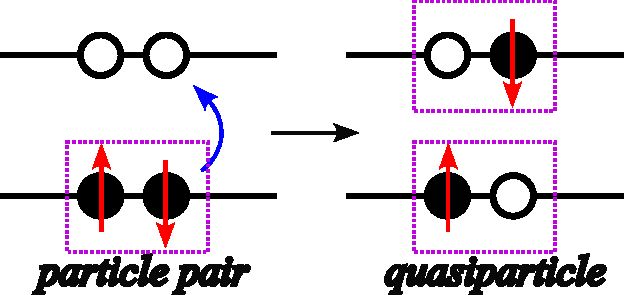
\includegraphics[scale=0.7]{figure/nuclear/particleToquasiparticle.pdf}
    \end{center}
    \caption{粒子对到准粒子态的变化。图中表示两准粒子激发。}\label{fig:partToquasipart}
\end{figure}


通过Bogoliubov–Valatin变换\cite{Bogoliubov1958,Valatin1961May}将粒子的产生和湮灭算符变换成准粒子的产生和湮灭算符
\begin{equation}\begin{aligned}
    a^{\dagger}_{\alpha} =& u_{a} c^{\dagger}_{\alpha} + v_{a} \tilde{c}_{\alpha} \\
    \tilde{a}_{\alpha} =& u_{a} \tilde{c}_{\alpha} - v_{a} c^{\dagger}_{\alpha}
    \label{eq:qp-crt-hil}
\end{aligned}\end{equation}

\begin{note}
    我们把准粒子产生算符作用到准粒子基态上
    $$a^{\dagger}_{\alpha} \Ket{BCS} = (u_{a} c^{\dagger}_{\alpha} + v_{a} \tilde{c}_{\alpha}) \Ket{BCS}$$
    $\Ket{BCS}$在轨道$\alpha$上已经有一定概率占据了一对粒子,因此$c^{\dagger}_{\alpha}\Ket{BCS} = 0$,而$\tilde{c}_{\alpha}$将湮灭$\Ket{BCS}$中的一个粒子并形成空穴。这样在原来的位置就将出现粒子-空穴对,这恰好是一个准粒子。

    准粒子湮灭算符作用到准粒子态上的结果推导详见\citep[P. 182 脚注]{zengjy}。
\end{note}

对于偶偶核基态或BCS真空态,核子是成对存在的,没有拆对的情况,因此没有准粒子。对于奇A核或奇奇核,存在粒子-空穴态,因此在BCS框架下是存在准粒子的。


\subsection{约束变分问题下的BCS}

\paragraph*{粒子数算符}

根据\citep[Eq. 13.38]{suhonen-NtoN},粒子数算符写为
\begin{equation*}\begin{aligned}
    \hat{n} = \sum_{\alpha}c^{\dagger}_{\alpha} c_{\alpha} =& \sum_{a} \hat{j}^2_{a} v_{a}^2 + \sum_{a} \hat{j}^2_{a} (u_{a}^2 - v_{a}^2) \left[a_{a}^{\dagger} \tilde{a}_a\right] \\
                                                            & + \sum_{a} \hat{j}_{a} u_{a} v_{a} \left([a_{a}^{\dagger} a_{a}^{\dagger}]_{00} - [\tilde{a}_{a}^{\dagger} \tilde{a}_{a}^{\dagger}]_{00}\right)
\end{aligned}\end{equation*}

上式只有常数项才对期望有贡献,因此将粒子数期望写为
\begin{equation}
    \bar{n} = \sum_{a} \hat{j}^2_{a} v_{a}^2
    \label{eq:bcs-part-oper}
\end{equation}

\begin{proof}
    我们取第二项进行计算,有
    \begin{equation*}
        \Braket{BCS|\sum_{a}\hat{j}^2_{a} (u_{a}^2 - v_{a}^2) \left[a_{a}^{\dagger} \tilde{a}_a\right]_{00}|BCS} = \sum_{a}\hat{j}^2_{a} (u_{a}^2 - v_{a}^2) \Braket{BCS| \left[a_{a}^{\dagger} \tilde{a}_a\right]_{00} |BCS}
    \end{equation*}
    由\citep[Eq. 2.51]{suhonen-NtoN},得关系
    \begin{equation*}
        \left[a_{a}^{\dagger} \tilde{a}_a\right]_{00} \sim \sum_{\alpha} a_{\alpha}^{\dagger} \tilde{a}_{\alpha} = \sum_{\alpha} a_{\alpha}^{\dagger} a_{-\alpha}
    \end{equation*}
    而费米子中角动量第三分量无法取到0,故不存在$\alpha = -\alpha$的情况,因此
    \begin{equation*}
        \Braket{BCS | a_{\alpha}^{\dagger} a_{-\alpha} | BCS} = 0
    \end{equation*}
    此项对粒子数算符无贡献。
\end{proof}



\bibliographystyle{modified-apsrev4-2}
\bibliography{reference}
